\chapter{弗里德曼膨脹、輻射與暗物質}

\section{基本宇宙學方程回顧}

在大於星系團的尺度上，宇宙可視為均勻的。選擇座標，使我們位於\(x=0\)，並將一個具代表性的星系，或單純視為隨哈伯流運動的假想粒子，置於\(x=1\)。依定義，它與我們的物理距離就是尺度因子\(a(t)\)。位於\(x=2\)的點距離我們\(2a(t)\)，依此類推。

\begin{figure}[ht]
\centering
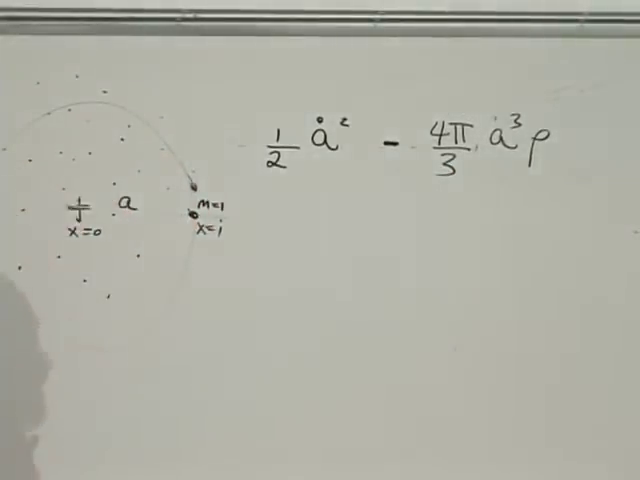
\includegraphics[width=0.78\textwidth]{lecture_03_figure_02.png}
\caption{以\(x=0\)為中心的均勻球體、位於\(x=1\)的共動星系，以及\(a(t)\)的牛頓力學能量平衡。}
\end{figure}

只有半徑為\(a(t)\)的球體內的物質，才會對位於\(x=1\)的粒子產生引力。令該粒子的質量為單位質量。它的動能為
\begin{equation}
\frac{1}{2}\dot a^2.
\end{equation}
球體內所含的質量為
\begin{equation}
M_{\mathrm{enc}}=\frac{4\pi}{3}a^3\rho,
\end{equation}
因此，引力位能為
\begin{equation}
-\frac{G M_{\mathrm{enc}}}{a}
=
-\frac{4\pi G}{3}a^2\rho.
\end{equation}
\editorialnote{在講課時間戳記00:05:30處，黑板上清楚寫出了動能項與依賴密度的位能項。此處列出的完整係數則是依據口頭推導補上。}

能量守恆給出
\begin{equation}
\frac{1}{2}\dot a^2-\frac{4\pi G}{3}a^2\rho=\text{const}.
\end{equation}
接著將常數記為\(-k\)；但要留意，只有將方程乘以\(2\)後，這個記號才符合標準正規化。在標準形式中，
\begin{equation}
\dot a^2=\frac{8\pi G}{3}a^2\rho-k,
\end{equation}
再除以\(a^2\)，得到
\begin{equation}
\left(\frac{\dot a}{a}\right)^2=\frac{8\pi G}{3}\rho-\frac{k}{a^2}.
\end{equation}
這就是本討論一貫使用的弗里德曼方程形式。

\begin{figure}[ht]
\centering
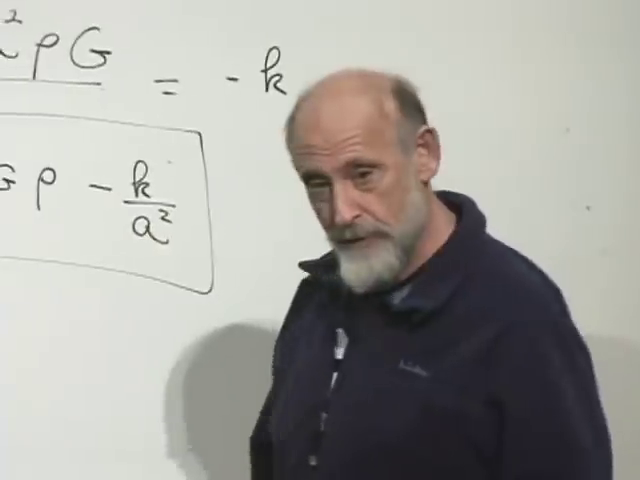
\includegraphics[width=0.56\textwidth]{lecture_03_figure_03.png}
\caption{弗里德曼方程中單獨標示出的曲率項\(-k/a^2\)。}
\end{figure}

觀測顯示，曲率項非常接近零；在這個層次上，將它忽略是相當好的近似。它確實代表空間曲率，但觀測到的效應太小，甚至無法判定曲率的正負。

同一個方程也可以從廣義相對論導出。示意而言，愛因斯坦方程的時間—時間分量為
\begin{equation}
R_{00}-\frac{1}{2}g_{00}R \propto T_{00}.
\end{equation}
\editorialnote{此處只列出張量結構，未列精確的整體數值係數。}
對於膨脹中的均勻度規，幾何側會產生\(\dot a/a\)與\(k/a^2\)的組合，物質側則是能量密度。就目前的討論而言，牛頓力學的論證與愛因斯坦方程描述的是同一件事。

這也改變了\(\rho\)的意義。從這裡開始，最好把\(\rho\)稱為能量密度。對共動參考系中緩慢運動的物質而言，它就是靜止能量密度。

\section{物質主導時期}

現在假設能量密度來自靜止於共動參考系中的物質。取一個座標邊長為一單位的立方體，其物理邊長為\(a(t)\)，因此物理體積為\(a^3(t)\)。若這個共動立方體內的質能為\(M\)，且物質隨著流動而不穿越立方體邊界，則
\begin{equation}
\rho_m=\frac{M}{a^3}.
\end{equation}

這就是物質主導的情形。在這個理想化模型中，粒子靜止於盒中，因此溫度視為零，壓力也視為零。要有壓力，粒子就必須穿越盒子的邊界。

令\(k\approx 0\)，方程便成為
\begin{equation}
\left(\frac{\dot a}{a}\right)^2=\frac{8\pi G}{3}\frac{M}{a^3}.
\end{equation}
試取冪次形式
\begin{equation}
a(t)=Ct^p.
\end{equation}
則
\begin{equation}
\frac{\dot a}{a}=\frac{p}{t},
\end{equation}
因此左側正比於\(t^{-2}\)，右側正比於\(t^{-3p}\)。比較冪次可得
\begin{equation}
3p=2,
\qquad
p=\frac{2}{3}.
\end{equation}
所以
\begin{equation}
a(t)\propto t^{2/3}.
\end{equation}
再比較係數可得
\begin{equation}
C^3=6\pi G M.
\end{equation}

這個解的重點在於冪次律。物質主導的宇宙，其膨脹與時間的三分之二次方成正比，而非線性正比。這個定律描述一段漫長的中間時期，約從大爆炸後\(10^5\)年開始，延續到幾十億年後。如今的宇宙並非嚴格由物質主導，因為暗能量目前占主導地位；不過，普通物質的行為以及宇宙歷史中很長的一段時期，都可以用這個模型描述。

\section{輻射主導時期}

在更早的時期，能量密度由輻射主導。原因很簡單：宇宙中有極大量的光子，每個質子大約對應\(10^9\)個光子；宇宙被壓縮時，這些光子的能量會升高。

光子沒有靜止質量，但有能量。其能量為
\begin{equation}
E_\gamma=h\nu=\frac{hc}{\lambda}.
\end{equation}
關鍵假設是，宇宙膨脹時，光子的波長也隨之伸長：
\begin{equation}
\lambda\propto a.
\end{equation}
盒中的波可以幫助理解這一點：盒子變大，波模的波長也隨盒子變長。這裡將相同的想法應用於膨脹中的宇宙。

由於\(\lambda\propto a\)，每個光子的能量正比於
\begin{equation}
E_\gamma\propto a^{-1}.
\end{equation}
再取一個共動的單位盒子。光子會進出盒子，但平均而言，盒內光子數維持不變。因此，盒內光子的總能量也正比於\(a^{-1}\)。再除以物理體積\(a^3\)，輻射能量密度便正比於
\begin{equation}
\rho_r\propto a^{-4}.
\end{equation}

多出的\(a^{-1}\)因子就是兩者的差異所在。宇宙膨脹會稀釋物質。輻射除了因膨脹而稀釋，每個光子還會因紅移而損失能量。

因此，輻射主導宇宙的弗里德曼方程為
\begin{equation}
\left(\frac{\dot a}{a}\right)^2=\frac{8\pi G}{3}\frac{M_r}{a^4}.
\end{equation}
\editorialnote{口頭講解中再次使用符號\(M\)表示這個新常數。此處加上\(r\)下標，只是為了與物質主導的情形區別。}

使用相同的試探形式\(a(t)=Ct^p\)。左側同樣正比於\(t^{-2}\)，右側則正比於\(t^{-4p}\)。比較冪次可得
\begin{equation}
4p=2,
\qquad
p=\frac{1}{2}.
\end{equation}
因此
\begin{equation}
a(t)\propto t^{1/2}.
\end{equation}
再比較係數可得
\begin{equation}
C^4=\frac{32\pi G}{3}M_r.
\end{equation}

\begin{classroomqa}
\lecturetimestamp{00:35:41}
\audiencequestion{為什麼裡面會有\(G\)？}
\lecturerresponse{因為產生引力效應的是能量密度，而不只是靜止質量。對緩慢運動的物質而言，這項差異很容易被忽略；但光子讓我們無法忽視這一點：光子沒有靜止質量，仍然會產生引力。}
\end{classroomqa}

裝滿輻射的盒子可以具體說明這一點。推動一個裝滿光子的盒子。盒子一旦加速，朝光子移動的盒壁受到的撞擊會比遠離光子的盒壁更強，因此必須更用力推，才能克服輻射壓。於是盒子有了額外的慣性；根據等效原理，這份額外慣性也代表額外的引力質量。這就是此處用來說明能量會產生引力的「光子盒」論證。

\begin{classroomqa}
\lecturetimestamp{00:38:11}
\audiencequestion{這兩個方程是否有任何一個存在\(a\)隨時間減小的解？}
\lecturerresponse{有。若把曲率項\(k/a^2\)加回去，就會有先膨脹再收縮的解。我們的宇宙看來並非如此演化，但方程確實允許這種解。}
\end{classroomqa}

\begin{classroomqa}
\lecturetimestamp{00:38:44}
\audiencequestion{那能量守恆呢？}
\lecturerresponse{若把\(k\)項加回去，並將方程乘回\(a^2\)，宇宙學方程正好就是守恆定律。方程一側的物質或輻射只是整體收支的一部分。膨脹也帶來動能與引力位能的部分，而總能量收支守恆。}
\end{classroomqa}

\section{物質與輻射並存}

真實的宇宙同時包含物質與輻射，兩者的密度隨尺度因子的變化不同：
\begin{equation}
\rho_m\propto a^{-3},
\qquad
\rho_r\propto a^{-4}.
\end{equation}
因此，\(a\)很小時由輻射主導；\(a\)很大時則由物質主導。往回追溯，早期宇宙必定由輻射主導。

\begin{figure}[ht]
\centering
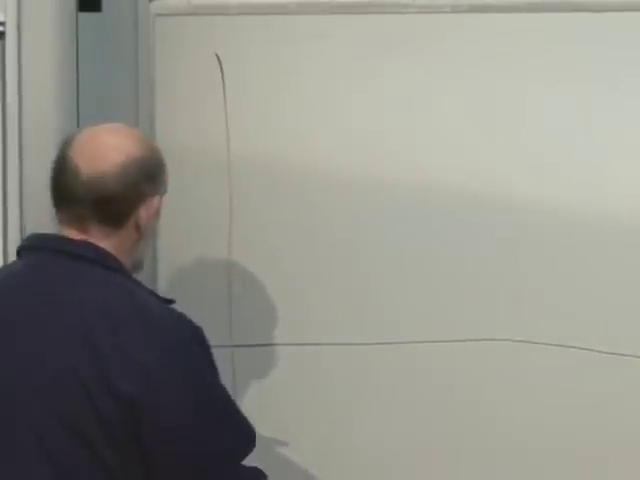
\includegraphics[width=0.68\textwidth]{lecture_03_figure_05.png}
\caption{比較物質與輻射能量密度隨尺度因子變化的座標軸。}
\end{figure}

\editorialnote{在講課時間戳記00：44：45處，黑板上只畫出了比較圖起始處的座標軸。緊接著討論的物質與輻射曲線只在正文中描述，並未在此重新繪出。}

物質曲線依\(a^{-3}\)的規律下降，輻射曲線則依\(a^{-4}\)的規律下降。當\(a\to 0\)時，兩者都發散，但輻射曲線在該處上升得更快，因此兩條曲線會在某個相等時的尺度因子處相交。粗略估計，這個轉變發生在大約\(10^4\)年後，或許還要稍久一些。

也可以用\(a(t)\)對\(t\)的圖來呈現同一件事。早期的膨脹行為類似\(t^{1/2}\)，後期則類似\(t^{2/3}\)。這項變化不是突然跳變，而是在相對狹窄的時間範圍內連續過渡。

\begin{classroomqa}
\lecturetimestamp{00:44:04}
\audiencequestion{隨著宇宙變老，冪次\(p\)會從\(1/2\)連續變為\(2/3\)嗎？}
\lecturerresponse{會。它不會突然跳變，而是連續改變，只是變化集中在相當狹窄的時間範圍內。}
\end{classroomqa}

\section{溫度、複合與最後散射}

接下來考慮溫度。若典型光子的能量正比於\(a^{-1}\)，輻射場的溫度也同樣如此：
\begin{equation}
T\propto a^{-1}.
\end{equation}
若\(a\)加倍，溫度就會減半。

取目前的光子溫度約為\(3\,\mathrm K\)，電離溫度約為\(3000\,\mathrm K\)，大致相當於太陽表面的溫度。則
\begin{equation}
\frac{a_{\mathrm{today}}}{a_{\mathrm{ion}}}\sim 10^3.
\end{equation}
使用晚期物質主導時期的定律\(a\propto t^{2/3}\)，
\begin{equation}
\left(\frac{t_{\mathrm{today}}}{t_{\mathrm{ion}}}\right)^{2/3}\sim 10^3,
\end{equation}
因此
\begin{equation}
\frac{t_{\mathrm{today}}}{t_{\mathrm{ion}}}\sim 1000^{3/2}\sim 3\times 10^4.
\end{equation}
以這項估算的精度，取宇宙年齡為\(10^{10}\)年，可得
\begin{equation}
t_{\mathrm{ion}}\sim 3\times 10^5\ \mathrm{years}.
\end{equation}

這是氫與氦不再完全電離的時期。在此之前，宇宙是高溫電漿。為什麼電漿不透明？因為自由電荷會強烈響應電磁波。電場驅使電荷來回運動，使介質表現得像導體；而導體是不透明的。這就是此處與太陽表面相比的原因。

宇宙冷卻到電子能與原子核複合後，普通的中性原子便形成，宇宙也變得透明許多。這項轉變並非在某個瞬間完成，而是發生於一段模糊的時間區間。不過對宇宙學而言，這段區間仍界定得夠清楚，因此稱為最後散射面。

向外看，就是回望過去。鄰近星系呈現的是較近的過去；更遙遠的星系則呈現更早的時期。距離夠遠時，每一條視線都會抵達宇宙仍處於電離、不透明狀態的時期。電磁輻射無法讓我們看到更早的宇宙。

原則上，其他信使可以探測更早的時期。中微子不帶電，會更早退耦。引力子若有朝一日能被觀測到，則會來自更早的時期。然而，正是讓它們能穿過早期電漿的微弱交互作用，也使它們極難探測。

如果宇宙曾經在各個方向上都像太陽表面一樣灼熱，為什麼天空沒有亮得令人目眩？因為最後散射面正在遠離我們，從那裡抵達的光子已經紅移了約\(10^3\)倍，恰好相當於\(3000\,\mathrm K\)與\(3\,\mathrm K\)之間的溫度比。抵達我們的是微波輻射，而不是可見光中的陽光。

\begin{classroomqa}
\lecturetimestamp{01:03:51}
\audiencequestion{所以我們的望遠鏡無法看到大約\(300{,}000\)年以前的宇宙嗎？}
\lecturerresponse{電磁望遠鏡無法做到。在那之前，宇宙處於電離且不透明的狀態。其他信使至少原則上能探測更早的時期。}
\end{classroomqa}

\begin{classroomqa}
\lecturetimestamp{01:08:43}
\audiencequestion{你說光子的溫度，是指具有該峰值輻射的黑體溫度。但這和波長並非線性關係，對吧？}
\lecturerresponse{沒錯。溫度本質上代表典型光子的能量，因此對光子而言，溫度與波長成反比。\(T^4\)定律描述的是能量密度，而非單一光子的能量；它結合了每個光子的能量與單位體積內的光子數，而光子數密度正比於\(T^3\)。}
\end{classroomqa}

因此
\begin{equation}
n_\gamma\propto T^3,
\qquad
\rho_\gamma\propto T^4.
\end{equation}

\section{從旋轉曲線推知暗物質}

暗物質的證據來自星系旋轉曲線。它並非從大尺度的弗里德曼方程推知，而是從星系尺度的天文觀測推知。

從最簡單的牛頓力學問題開始：質量為\(m\)的輕質物體，以\(M\)為中心質量，在半徑\(r\)處繞行。引力大小為
\begin{equation}
\frac{GMm}{r^2},
\end{equation}
向心加速度則為\(v^2/r\)。牛頓定律給出
\begin{equation}
m\frac{v^2}{r}=\frac{GMm}{r^2}.
\end{equation}
約去\(m\)，再乘以\(r\)，可得
\begin{equation}
v(r)=\sqrt{\frac{GM}{r}}.
\end{equation}
所以，若引力質量集中在中心附近，軌道速度便會依\(r^{-1/2}\)的規律下降。

如果質量分布跟著光的分布，這正是預期的結果。星系中大部分可見物質位於核心附近，因此外圍恆星的運動應類似外太陽系中的行星。天文學家測量鄰近星系兩側的多普勒位移差異，以推知軌道速度：先扣除整個星系的退行運動，再比較朝我們運動的一側與遠離我們的一側。觀測到的軌道速度在很大的半徑範圍內仍大致不變。

因此，將中心質量\(M\)換成半徑內的總質量\(M(r)\)：
\begin{equation}
\frac{v^2}{r}=\frac{G M(r)}{r^2}.
\end{equation}
若\(v(r)\)近似不變，則
\begin{equation}
M(r)\propto r.
\end{equation}
換句話說，即使可見光不再增加，引力質量仍會隨半徑持續增加。

現在依照此處為求簡化所採用的假設，令質量分布大致呈球對稱。則
\begin{equation}
M(R)=\int_0^R 4\pi r^2\rho(r)\,dr.
\end{equation}
若\(M(R)\propto R\)，對\(R\)微分可得
\begin{equation}
4\pi R^2\rho(R)\propto 1,
\end{equation}
因此
\begin{equation}
\rho(r)\propto \frac{1}{r^2}.
\end{equation}

\begin{classroomqa}
\lecturetimestamp{01:28:18}
\audiencequestion{看起來密度應該正比於\(1/r^2\)。這是有原因的嗎？}
\lecturerresponse{從觀測到的平坦旋轉曲線可推得\(M(R)\propto R\)，再微分便得到\(\rho(r)\propto 1/r^2\)。除此之外，此處並未提出簡單的第一原理解釋；詳細模擬在這方面發揮了很大作用。}
\end{classroomqa}

可以確定的是，星系的引力質量遠大於僅從發光物質推算出的質量，大約多出數倍；依此處採用的估計，則約多出一個數量級。可見星系位於大得多的暗物質暈之中。

為什麼普通氣體不會維持在這種稀薄狀態？原因是耗散。氣體雲會收縮，是因為碰撞、類似摩擦的過程以及輻射讓它能量逐漸流失。暗物質顯然不會顯著輻射，而且幾乎不發生碰撞。引力可以將它向內拉，並把位能轉換成動能；但若沒有有效的耗散，它就不會坍縮成普通物質形成的緻密發光結構。維持暗物質暈延展的，是動能。

接著謹慎地討論了幾種替代可能。中微子的速度太快，無法在星系尺度上形成這樣的結構。由普通氫構成的暗物質暈會嚴重影響早期宇宙的核合成。由普通物質形成的黑洞也有問題，因為這代表早期宇宙中的普通物質過多，並會帶來引力透鏡方面的問題；此處的討論並未進一步主張其他結論。

暗物質暈並非薄殼或環面，而是一個近似球形、密度不均的球體：中心較密，往外逐漸變稀。

\begin{classroomqa}
\lecturetimestamp{01:53:12}
\audiencequestion{你說的是子彈星系團嗎？}
\lecturerresponse{是。X射線氣體顯示普通物質的分布，引力透鏡則顯示總引力質量的分布。在這次碰撞中，兩者分離了。這是暗物質確實存在的有力證據，而非僅僅修改與可見物質相關的引力理論。}
\end{classroomqa}

這就是最後一項觀測重點。人們對暗物質本質的細節所知甚少，但此處的論述不需要引入激進的新原理。一種保守的可能性是，自然界中還有尚未辨識出的弱交互作用粒子。